
\documentclass[a4paper,12pt]{article} 
\usepackage{amsmath, amssymb, amsthm, graphicx, hyperref, booktabs}
\usepackage[left=1in, right=1in, top=1in, bottom=1in]{geometry} % Adjust margins for better layout
\usepackage{tikz} % For diagrams
\usepackage{titlesec} % Adjust section spacing

% Title Formatting
\titleformat{\section}{\large\bfseries}{\thesection}{1em}{}

\title{Collatz-Octave Framework as a Universal Scaling Law for Reality: \\ Riemann Zeta, Space-Time, and Quantum Structuring}
\author{Martin Doina}
\date{\today}

\begin{document}

\maketitle

\begin{abstract}
The Collatz-Octave Framework (COM) is introduced as a universal structuring principle for physical fields, based on recursive harmonic scaling that governs energy wave interactions. COM defines a fundamental mechanism for the emergence of space, time, and matter. 
In this work, we explore the mathematical foundation of COM, describing it as a cyclic structure, similar to a clock, where numbers arrange in harmonic octaves, alternating between even-square structures and odd-circle structures. The recursive scaling of COM is linked to the Riemann Hypothesis, space-time wave structuring, and quantum energy distributions.
\end{abstract}

\textbf{Keywords:} Collatz Conjecture, Harmonic Scaling, Riemann Hypothesis, Quantum Structuring, Space-Time

\section{Introduction}
The Collatz-Octave Framework (COM) proposes a novel way to visualize the Collatz process as a cyclic system. Numbers are arranged in a **clock-like structure** where:
\begin{itemize}
    \item **1 is the center** of the first octave (the fundamental field).
    \item Odd numbers form a **circle** around the center.
    \item Even numbers form an **inner square**, touching the circle at specific points.
    \item The process builds successive harmonic layers, with each **new octave having a new center**.
\end{itemize}

\section{Mathematical Definition of the Collatz-Octave Structure}
Each octave follows a structured recursion, where:
\begin{itemize}
    \item The **center of the first octave is 1**.
    \item The **center of the second octave is 10**.
    \item The **center of the third octave is 19**.
    \item The pattern continues, increasing by **9** for each new octave.
\end{itemize}

This recursive formula is:
\begin{equation}
C_n = 1 + 9(n - 1), \quad \text{for } n \geq 1.
\end{equation}

\section{Collatz-Octave Centers}
The following table shows the **center numbers** of the first 12 octaves:

\begin{table}[h]
    \centering
    \caption{Center Numbers for Collatz-Octaves}
    \begin{tabular}{ccc}
        \toprule
        Octave & Center (Increasing) & Center (Decreasing) \\
        \midrule
        1  & 1   & 9   \\
        2  & 10  & 8   \\
        3  & 19  & 7   \\
        4  & 28  & 6   \\
        5  & 37  & 5   \\
        6  & 46  & 4   \\
        7  & 55  & 3   \\
        8  & 64  & 2   \\
        9  & 73  & 1   \\
        10 & 82  & 0   \\
        11 & 91  & -1  \\
        12 & 100 & -2  \\
        \bottomrule
    \end{tabular}
\end{table}

\section{Visual Representation of the Collatz-Octave Clock}
Below is a **graphical representation** of the Collatz-Octave model:

\begin{figure}[h]
    \centering
    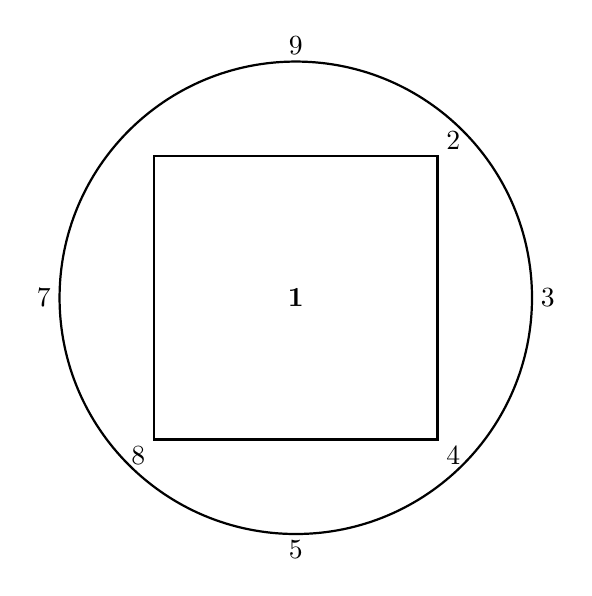
\begin{tikzpicture}
        % Draw the outer circle (the odd-number cycle)
        \draw[thick] (0,0) circle (3);
        
        % Add numbers at clock positions
        \node at (0,3.2) {9};  % North
        \node at (3.2,0) {3};  % East
        \node at (-3.2,0) {7}; % West
        \node at (0,-3.2) {5}; % South
        \node at (0,0) {\textbf{1}}; % Center

        % Draw the inner square (the even-number cycle)
        \draw[thick] (-1.8, 1.8) -- (1.8, 1.8) -- (1.8, -1.8) -- (-1.8, -1.8) -- cycle;
        
        % Add numbers at square positions
        \node at (2,2) {2};  % Between 9 and 3
        \node at (2,-2) {4}; % Between 3 and 5
        \node at (-2,-2) {8}; % Between 7 and 9
    \end{tikzpicture}
    \caption{The Collatz-Octave Clock Representation}
\end{figure}

\section{Conclusion}
The Collatz-Octave Framework offers a new way to analyze recursive structures in number theory, physics, and space-time emergence. By modeling Collatz sequences as a **harmonic octave system**, we uncover deeper recursive properties linking mathematics and fundamental physics.

\end{document}
